\section{Задание 1}

Создайте объект, в котором блоковый элемент размерами 250 на 250 и заливкой красного цвета заключён в рамку тёмно-синего цвета типа inset и толщиной 10. По нажатию кнопки изменять цвет заливки на голубой и надпись на кнопке. При следующем нажатии изменять цвет заливки на красный и надпись на кнопке.

\begin{center}
  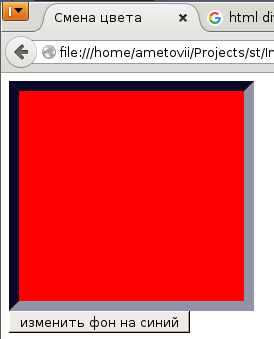
\includegraphics{img/Exercise_01/01.png}
  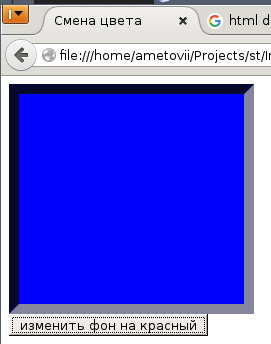
\includegraphics{img/Exercise_01/02.png}
  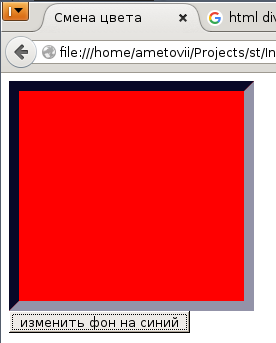
\includegraphics{img/Exercise_01/03.png}
\end{center}

Исходный код \verb|exercise_01.html|:

\begin{verbatim}
<!DOCTYPE HTML>
<html>
  <head>
    <meta charset="utf-8">
    <title>Смена цвета</title>
    <style type="text/css">
      .block1 {
      width: 250px;
      height: 250px;
      background: red;
      padding: 5px;
      padding-right: 20px;
      border: inset 10px #0b0b3b;
      float: left;
      }
      
      .block2 {
          width: 100%;
          height: auto;
	  float: left;
      }
    </style>
    <script>
      function changeColorLabel(){
	  var myButton=document.getElementById('button');
	  var myDiv=document.getElementById('changedDiv');
	  if (myButton.value=="изменить фон на синий"){
	      myButton.value="изменить фон на красный";
	      myDiv.style.background="blue";
	  }
	  else{
	      myButton.value="изменить фон на синий";
	      myDiv.style.background="red";}
      }
    </script>
  </head>
  <body>
      <div class="block1" id='changedDiv'></div>
      <div class="block2"><input type="button"
				 id='button'
				 onClick="changeColorLabel();"
				 value="изменить фон на синий"/></div>
  </body>
</html>
\end{verbatim}
